\chapter{Design and Implementation}
\label{chap:implementation}

Overview... Architecture... General Components

\section{Initial Situation}
Currently the data which should be analyzed is available through the protocols of the sessions of the national council. These protocols are publicly available and can be found at the website of the Austrian parliament (See \url{https://www.parlament.gv.at/PAKT/STPROT/}). They are in PDF-format and since the $20^{th}$ legislative period also available in HTML. As the extracting of the PDF-files would not result in sufficient quality, in this thesis only the data since the $20^{th}$ legislative period is being extracted and analyzed.

\subsection{Current Data Structure}
asdf

\section{Overall Process}
Figure \ref{fig:general_architecture} shows the general Architecture of the prototype which was implemented.

\begin{figure}
	\centering
	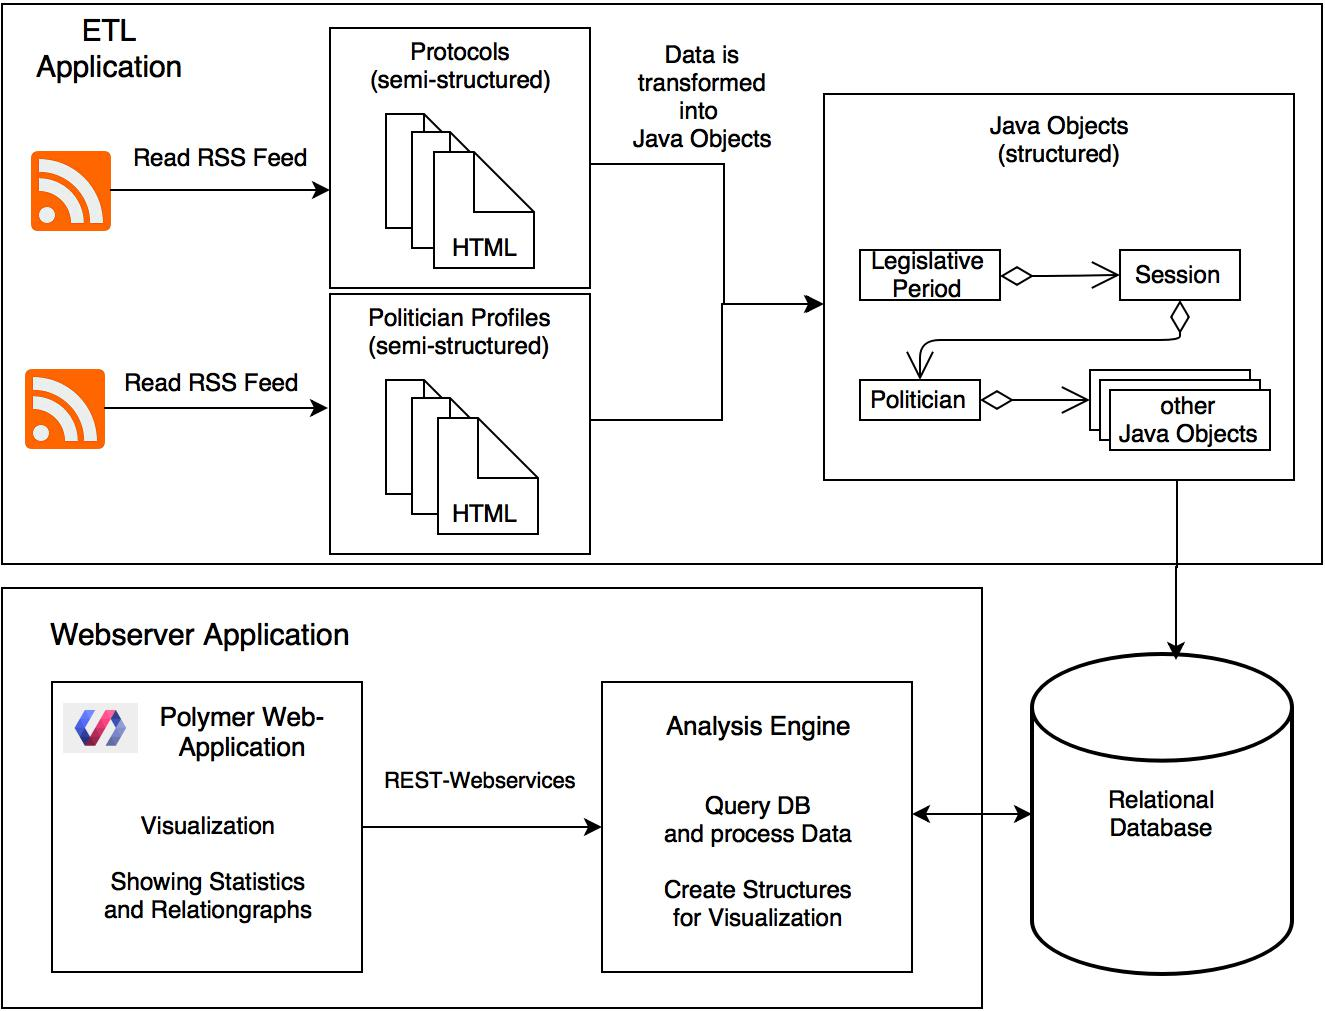
\includegraphics[width=\textwidth]{imgs/overall_architecture}
	\caption{General Architecture}
	\label{fig:general_architecture}
\end{figure}

\section{Data Extraction and Transforming}
\label{sec:data_extraction_transforming}

\section{Export into Database}
\label{sec:export_db}

\section{Analysis}
\label{sec:analysis}

\section{Visualization}
\label{sec:visualization}
